\documentclass[10pt,usepdftitle=false,aspectratio=169]{beamer}
% \documentclass[10pt,usepdftitle=false,aspectratio=169,handout]{beamer}

\usepackage{subfig}
\usepackage{graphicx}
\graphicspath{{../Figures/}}

\input{preamble_talk}
% \input{../preamble_slides}
\usepackage{tcolorbox}
\usepackage{changepage}
\usepackage{arydshln}       %for dashed lines

% Assets included in preamble
\newcommand{\assetsDIR}{assets}

% Add speaker notes to talk
% \setbeameroption{hide notes} % Only slides
%\setbeameroption{show only notes} % Only notes
% \setbeameroption{show notes on second screen}

\usetikzlibrary{external}
\usetikzlibrary{positioning}
\tikzset{main node/.style={circle,fill=white,draw,minimum size=1cm,inner sep=0pt},}
% \tikzexternalize[mode=list and make]
% use  make -j 4 -f talk.makefile to compile with 8 parallel threads (this is what it takes to max out the machine, depsite it having 4 cores)
\tikzset{external/force remake=false}
\tikzsetexternalprefix{external/}

\usepackage[super]{nth}
\newcommand{\LargeFigure}[1]{\begin{figure}
\includegraphics[width=\textwidth,height=0.95\textheight,keepaspectratio]{#1}
\end{figure}}

%\setbeamersize{text margin left=0pt,text margin right=0pt} 
\begin{document}

\tikzexternaldisable

% %%%%%%%%%%%%%%%%%%%%%%%%%%%%%%%%%%%%%%%%%%%%%%%%%%%%%%%%%%%%%%%%%%%%%%%%%%%%%%%%%%%%%%%%%
% %                                     TITLE                                             %
% %%%%%%%%%%%%%%%%%%%%%%%%%%%%%%%%%%%%%%%%%%%%%%%%%%%%%%%%%%%%%%%%%%%%%%%%%%%%%%%%%%%%%%%%%

\begin{frame}
  \title{{\bf Intermediate Summary of Wasserstein tSNE}\\[4mm]{}
  \vspace*{-.7cm}}
  \author{Fynn Bachmann \vspace{-1cm}} \date{June \nth{17}, 2021}

  \vspace{-1.5cm}
  \maketitle
  \vspace{-1.0cm}

  \begin{columns}
    \column{0.45\textwidth}
    \includegraphics[width=\textwidth]{\assetsDIR/UT_WBMW_Rot_RGB.pdf}\hfill
    % \column{.45\textwidth}
    \column{0.45\textwidth}
    \dre{Faculty of Science\\
    Department of Computer Science\\
    {\small Chair for the Methods of Machine Learning}}
    % \includegraphics[width=.8\textwidth]{\assetsDIR/MPI-IS-WortBildMarke.png}\\
    % \includegraphics[width=.8\textwidth]{\assetsDIR/imprs-is-logo.pdf}\\
    % \parbox[c]{.2\textwidth}{\centering\includegraphics[height=1.2cm]{\assetsDIR/ERC.png}}
    % \parbox{.75\textwidth}{\scriptsize \color{ERC_ora}some of the presented work is supported\newline by the European Research Council.}
  \end{columns}

  \thispagestyle{empty}
  \setcounter{framenumber}{0}

  %%%%%%%%%%%%%%%% ANIMATED LOGO %%%%%%%%%%%%%%%%
  % \tikzifexternalizing{}{%
  % \begin{tikzpicture}[remember picture,overlay]
  % \node[anchor=south,yshift=-5mm] at (current page.south)
  % {\animategraphics[width=0.9995\paperwidth,autoplay,loop]{36}{\assetsDIR/logo_TU_169_}{0}{39}};
  %   \end{tikzpicture}%
  % }%
  %%%%%%%%%%%%%% END OF ANIMATED LOGO %%%%%%%%%%%

  %%%%%%%%%%%%%%%% STATIC LOGO %%%%%%%%%%%%%%%%%%
  \tikzifexternalizing{}{%
  \begin{tikzpicture}[remember picture,overlay]
   \node[anchor=south,yshift=-5mm] at (current page.south)
  {\includegraphics[width=0.9995\paperwidth]{\assetsDIR/logo_TU_169_1.pdf}};
  \end{tikzpicture}%
  }%
  %%%%%%%%%%%%%% END OF STATIC LOGO %%%%%%%%%%%%%

\end{frame}
\tikzexternalenable

\setlength{\figurewidth}{\textwidth}
\setlength{\figureheight}{\textheight}

% %%%%%%%%%%%%%%%%%%%%%%%%%%%%%%%%%%%%%%%%%%%%%%%%%%%%%%%%%%%%%%%%%%%%%%%%%%%%%%%%%%%%%%%%%
% %                                     INTRO                                             %
% %%%%%%%%%%%%%%%%%%%%%%%%%%%%%%%%%%%%%%%%%%%%%%%%%%%%%%%%%%%%%%%%%%%%%%%%%%%%%%%%%%%%%%%%%

%%%%%%%%%%%%%%%%

\begin{frame}\frametitle{Topic Description}
   \begin{prob}
   We want to find out in which sense a "Wasserstein t-SNE" can be useful. Which datasets exist where each datum itself is a probability distribution? How are they visualized/clustered now, and which metrics on probability distributions can improve clustering?
   \end{prob}
\end{frame}

%\begin{frame}{Overview}
%\begin{multicols}{2}
%\tableofcontents
%\end{multicols}
%\end{frame}


\section[HGM]{Hierarchical Gaussian Mixtures}


\begin{frame}{Hierarchical Gaussian Mixtures}
\begin{block}
\justifying Let $\mathcal{U}, \mathcal{N}, \mathcal{W}$ be Uniform, Normal and Wishart distributions respectively. A Hierarchical Gaussian Mixture is then defined by:
\end{block}
\begin{center}
 \begin{minipage}{11cm}
 \begin{itemize}
    \item[F Features] %$F\in\mathbb{R}$
    \item[K classes] $C_k = (s_k, \Lambda_k, \nu_k, \Gamma_k) $ %with $s_k\in\mathbb{R}, \Lambda_k \in \mathbb{R}^{F\times F }, \nu_k\in \mathbb{R}^{F}, \Gamma_k\in \mathbb{R}^{F\times F})$
    \item[N datapoints] ($D_{n})_k = (\mu_n, \Sigma_n)_k$ with $\mu_n \sim \mathcal{N}(\nu_k ,\,\Gamma_k)$ and $\Sigma_n \sim \mathcal{W}(s_k, \,\Lambda_k)$
    \item[M Samples] $(S_{m})_n \sim \mathcal{N}(\mu_n,\,\Sigma_n)$
\end{itemize}
\end{minipage}
\end{center}
\begin{block}{For now:}
\justifying
 Random models with $F=2$ and hyperparameters $a,b \in \mathbb{R}_+$\\
 $s_k \sim \mathcal{U}([F,\infty])$, \quad $\nu_k \sim \mathcal{U}([-a,a]^F)$, \quad $\Gamma_k \sim \mathcal{W}(F, \,b\cdot\mathbb{1}_F)$, \quad and $\Lambda_k \sim \mathcal{W}(F, \,\mathbb{1}_F)$
\end{block}
\end{frame}


\subsection{Synthetic Data}

\begin{frame}{}
\begin{figure}
\includegraphics[height=\textheight]{HGM/RandomHGM.pdf}
\end{figure}
\end{frame}

\subsection{Wasserstein tSNE}

\begin{frame}{Wasserstein t-SNE}
\begin{block}{Formal Definition:}
\justifying
$W(\mu_{1}, \mu_{2})^{2} :=\left\|m_{1}-m_{2}\right\|_{2}^{2}+\text { trace }\left(C_{1}+C_{2}-2\left(C_{2}^{1 / 2} C_{1} C_{2}^{1 / 2}\right)^{1 / 2}\right)$
\end{block}

Now we introduce a hyperparameter $w \in [0,1]$, that puts emphasis either on means or covariances.

\begin{block}{Convex Generalization:}
\justifying
$W(\mu_{1}, \mu_{2})^{2} := (1-w) \cdot \left\|m_{1}-m_{2}\right\|_{2}^{2}+ w \cdot  \text { trace }\left(C_{1}+C_{2}-2\left(C_{2}^{1 / 2} C_{1} C_{2}^{1 / 2}\right)^{1 / 2}\right)$
\end{block}
\end{frame}



\begin{frame}{}
\begin{figure}
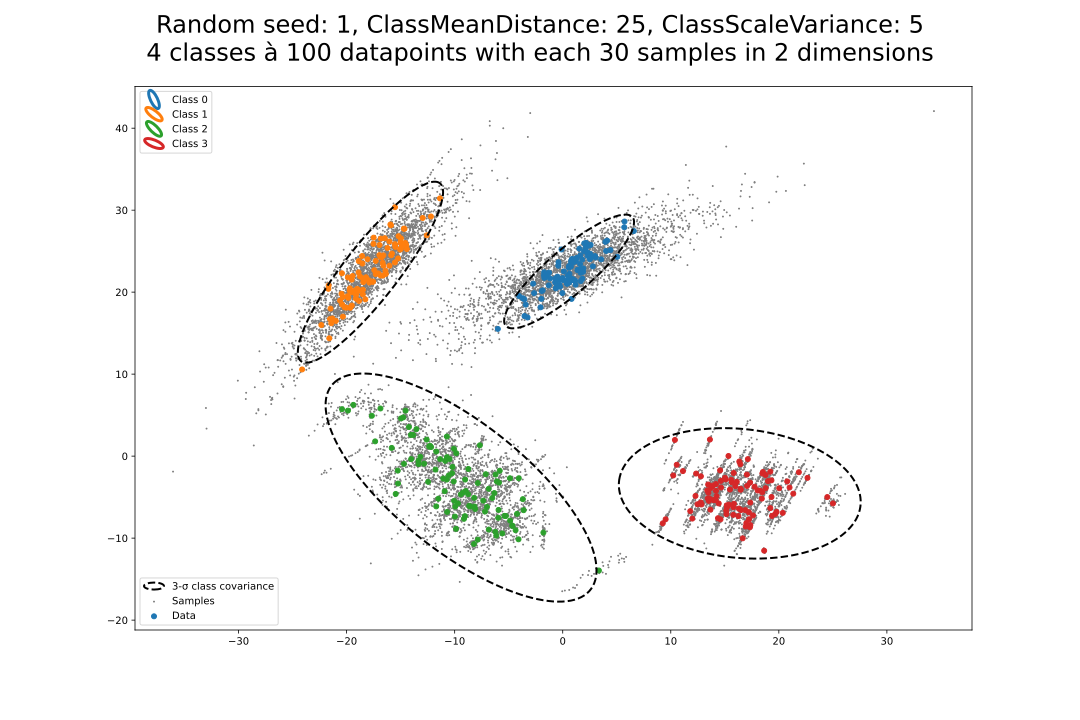
\includegraphics[width=\textwidth,height=\paperheight,keepaspectratio]{HGM/CleanExample}
\end{figure}
\end{frame}

\begin{frame}{}
\begin{figure}
\includegraphics[width=\textwidth]{HGM/RandomExample.pdf}
\end{figure}
\end{frame}



\section[EVS]{European Values Study}

\begin{frame}{European Values Study}
 \begin{itemize}
    \item 37688 interviews from 114 European NUTS-1 regions
    \item 20 questions per interview with options from 1 and 10
    \item variety of different topics (i.e. environment, democracy, morality)
    \item 34 countries as labels (classes)
\end{itemize}
\end{frame}

\begin{frame}{TSNE Embedding of NUTS1 regions}
\begin{figure}
\includegraphics[width=0.95\textwidth]{EVS/Embedding.pdf}
\end{figure}
\end{frame}

\subsection{Analysis}


\begin{frame}{Covariance Analysis}
\begin{figure}
\includegraphics[width=0.95\textwidth]{EVS/Covariances.pdf}
\end{figure}
\end{frame}


\begin{frame}{Correlation}
\begin{figure}
\includegraphics[width=0.95\textwidth]{EVS/Correlation.pdf}
\end{figure}
\end{frame}



\begin{frame}{}
\begin{figure}[!ht]
  {\includegraphics[width=.95\textwidth]{EVS/FeatureMeans.pdf}}\\
  {\includegraphics[width=.95\textwidth]{EVS/FeatureStds.pdf}}
\end{figure}
\end{frame}


\subsection{Questions}


\begin{frame}{Problems \& Questions}
 \begin{itemize}
    \item Logit Transformation doesn't make difference
    \item 
\end{itemize}
\end{frame}

\section[GER]{Bundestagswahl 2017}


\begin{frame}{Bundestagswahl 2017}
 \begin{itemize}
    \item 88499 Wahlbezirke from 299 Wahlkreise 
    \item 6 features (voting results of major parties)
    \item 16 federal states as labels
\end{itemize}
\end{frame}


\begin{frame}{}
\begin{figure}
\includegraphics[width=0.95\textwidth]{GER/Embedding.pdf}
\end{figure}
\end{frame}


\subsection{Analysis}


\begin{frame}{Covariance Analysis}
\begin{figure}
\includegraphics[width=0.95\textwidth]{GER/Covariances.pdf}
\end{figure}
\end{frame}


\begin{frame}{Correlation}
\begin{figure}
\includegraphics[width=0.95\textwidth]{GER/Correlation.pdf}
\end{figure}
\end{frame}


\begin{frame}{}
\begin{figure}[!ht]
  {\includegraphics[width=.95\textwidth]{GER/FeatureMeans.pdf}}\\
  {\includegraphics[width=.95\textwidth]{GER/FeatureStds.pdf}}
\end{figure}
\end{frame}


\subsection{Questions}

\begin{frame}{Problems \& Questions}
 \begin{itemize}
    \item Feature mean correlates with Feature variance
\end{itemize}
\end{frame}

\section[BIG5]{Big Five Personality Traits}


\begin{frame}{Bundestagswahl 2017}
 \begin{itemize}
    \item 219584 survey participants from 120 countries 
    \item 50 questions (answers options from 1 to 5)
    \item 5 continents as labels
    \item strong bias in an online survey (students only?)
\end{itemize}
\end{frame}

\begin{frame}{}
\begin{figure}[!ht]
  {\includegraphics[width=.95\textwidth]{BIG5/EmbeddingCountries.pdf}}\\
  {\includegraphics[width=.95\textwidth]{BIG5/EmbeddingContinents.pdf}}
\end{figure}
\end{frame}


\subsection{Analysis}


%\begin{frame}{Covariance Analysis}
%\begin{figure}
%\includegraphics[width=0.95\textwidth]{BIG5/Covariances.pdf}
%\end{figure}
%\end{frame}


\begin{frame}{Correlation}
\begin{figure}
\includegraphics[height=0.95\textheight]{BIG5/Overview.pdf}
\end{figure}
\end{frame}

\begin{frame}{}
\begin{figure}[!ht]
  {\includegraphics[width=.95\textwidth]{BIG5/FeatureMeans1.pdf}}\\
  {\includegraphics[width=.95\textwidth]{BIG5/FeatureMeans2.pdf}}
\end{figure}
\end{frame}


\subsection{Questions}

\begin{frame}{Problems \& Questions}
 \begin{itemize}
    \item No improvement with Wasserstein t-SNE
\end{itemize}
\end{frame}






\end{document}

